\subsection{Flavour in the SM}
% The Standard Model is a theory that contains particle fields, ordinary matter is composed of and messenger fields mediating interactions between them. 
% These fields can be separated by their quantum numbers indicating their couplings to each other. At first we have the twelve gauge vector boson fields, 
% eight gluon fields $G_a$ for strong interactions with coloured ($C$) particles and four electroweak boson fields $W_1$, $W_2$, $W_3$ and $B$ which couple
% to particles with weak isospin $T$ and hypercharge $Y_W$ respectively. Now we have 24 fermion fields, six leptons and six quarks each carrying one of three colours.
% The leptons can be subdivided into three electrically ($Q=T+Y_W$) charged and three uncharged ones and the quarks into three up-type ($T=\sfrac12$) and
% three down-type ($T=-\sfrac12$). Last but not least, the already mentioned scalar Higgs-field $\phi$ which develops a non vanishing vacuum expectation value
% (vev) $v$. This is the source for the spontanious breaking of the electroweak symmetry into the electromagnetic 
% (NOT)
The Standard Model is a gauge quantum field theory whose internal symmetry is the unitary product group $\mathcal{G}_\text{SM}=SU(3)_C\times SU(2)_L\times U(1)_{Y_W}$ representing
the quantum chromodynamics (QCD) whose charge is called color $C$ and the electroweak theory (GSW-Theory) whose charges are the weak isospin $T$ 
(hold by left handed particles) and the weak hypercharge $Y_W$ (\cite{Peskin}\cite{MDSchwartz}\cite{Langacker} for reviews). 
\\ \\ \textit{Particle content}\\
\noindent These quantum numbers (QN) are carried by a set of particle fields, ordinary matter is composed
of and messenger fields mediating these interactions between them. In particular twelve gauge vector boson fields, eight gluon fields $G^A_\mu$ ($A=1,2,...,8$)
for strong 
interactions and four electroweak boson fields from which $W^a_\mu$ ($a=1,2,3$) couple to the weak isospin and $B_\mu$ to the weak hypercharge. Now we have 12
fermion fields, six leptons $e$, $\mu$, $\tau$ as well as their respective neutrinos $\nu$ and six quarks $u$, $d$, $s$, $c$, $b$, and $t$. Actually there
are even more since they are defined by their QN. So for each fermion there is a distinction drawn between left handed $f_L$ ($T=\sfrac12$) and right 
handed $f_R$ ($T=0$), $f=f_L+f_R$. The left handed fields form isospin doublets as $Q_L=(u_L,d_L)$
and $L_L(e_L,\nu_L)$. Furthermore there are three different colours for each quark. 
Finally, there is the complex scalar field $\phi$ of the already mentioned Higgs-boson which is required for conservation of gauge invariance 
that would be broken by the mass terms of the other particles.
% Finally the field 
% $\phi$ of the already mentioned scalar
% Higgs-boson holds a special role in the SM. 
% It is known that the boson fields physical $W^\pm$ and $Z$, responsible for weak processes, have nonzero masses. But their
% mass terms would break the gauge invariance of the Lagrangian. So the Higgs-mechanism was considered wherein $\phi$ develops a non vanishing vacuum expectation
% value $\langle\phi\rangle$ (vev) which breaks the electroweak symmetry spontaniously (SSB) down to the electromagnetic symmetry $U(1)_Q$ resulting in a still massless photon field 
% $A$ and the three just named massive ones as superpositions of the four massless ones.
\subsubsection{Standard Model Interactions}
The Lagrangian to $\mathcal{G}_\text{SM}$ without gauge fixing and ghosts reads as
\begin{align}
 \mathcal{L}_\text{SM} &= \bar \psi \ti \slashed{D}\psi -y\bar\psi_L\phi\psi_R \nonumber\\
 &- \frac14\left[G^A_{\mu\nu}G^{A,\mu\nu} + W^a_{\mu\nu}W^{a,\mu\nu} + B_{\mu\nu}B^{\mu\nu}\right] - \left(D_\mu\phi\right)^*\left(D^\mu\phi\right) - V(\phi)    
 \label{eq_smlagrange}
\end{align}
where the terms represent the gauge interaction, the Yukawa interaction, the messenger propagation, the Higgs gauge interaction and
the Higgs potential, respectively. The covariant derivative $\slashed{D}=D^\mu\gamma_\mu$ is
\begin{align}
 D_\mu = \partial_\mu -\ti g_s G^A_\mu \lambda_A - \ti g W^a_\mu\sigma_a - \ti g'B_\mu
\end{align}
with the respective couplings $g_s$, $g$, $g'$ and group generators $\lambda$, $\sigma$. The field strength tensors are
\begin{align}
 G^A_{\mu\nu} = \partial_\mu G^A_\nu - \partial_\nu G^A_\mu + g_s f^{ABC}G^B_\mu G^C_\nu,\\
 W^a_{\mu\nu} = \partial_\mu W^a_\nu - \partial_\nu W^a_\mu + g \epsilon^{abc}W^b_\mu W^c_\nu,\\
 B_{\mu\nu} = \partial_\mu B_\nu - \partial_\nu B_\mu.
\end{align}
As messenger of an abelian $U(1)_Y$ there are no self-interactions for $B$, whereas, for messengers of the non-abelian ones $G$ and $W$ interact 
with themselves whose amplitude is expressed with the connection $f$, $\epsilon$. Mass terms for fermions $\bar\psi_R m\psi_L + \bar\psi_L m\psi_R$ 
break gauge invariance since $\psi_L$ and $\psi_R$ have different representations under the electroweak symmetry group. 
\\ \\ \textit{Yukawa Interaction} \\
\noindent In order to assign a 
mass to them, the electroweak symmetry gets broken spontaneously (SSB) by the Higgs-mechanism. The Higgs field is a doublet under the $SU(2)_L$ which 
develops 
a real vacuum expectation value $\langle \phi\rangle \propto (0,v)$ minimising its potential $V(\phi)=-\mu^2|\phi|^2+\lambda|\phi|^4$, so that
$v\propto\sqrt{\mu^2/\lambda}$. 
SM gauge interactions do not differ between the fermion generations which is why we introduce the vectors
$u=(u,c,t)$, $d=(d,s,b)$ and $e=(e,\mu,\tau)$ in family space. The origin of the experimentally observed neutrino masses is yet unknown since
no right handed neutrinos are considered in the SM but could be added as well in a minimal extension and afterwards treated alike.
The Yukawa interaction after SSB reads as
\begin{equation}
 \mathcal{L}_m = -v \bar u^i_L y^u_{ij}u^i_R -v \bar d^i_Ly^d_{ij} d^i_R -v \bar e^i_Ly^e_{ij} e^i_R + \text{h.c.}
 \label{eq_massSM}
\end{equation}
with $y^u$, $y^d$ and $y^e$ being $3\times 3$ ($i,j=1,2,3$) real, Yukawa matrices. $\phi^c = \ti\sigma_2\phi^*$ is the charged conjugate 
Higgs. 
The $y^\alpha$, ($\alpha=u,d,e$) are in general not diagonal but particles are measured to have a distinct mass value. Therefore they are expressed
in the mass basis due to bidiagonalisation with two unitary matrices $V_\alpha$, $U_\alpha$. Exemplarily for the first term in \eqref{eq_massSM}
it becomes
\begin{align}
 \mathcal{L}_m \supset -v u_L V_u^\dagger V_u y_u U^\dagger_u U_u u_R = -v u'_L \hat{y}_u u'_R.
 \label{eq_diracmass}
\end{align}
The masses $m_\alpha$ enter through $m_\alpha = v\hat{y}_\alpha$ with the hierarchies
\begin{equation}
\begin{aligned}
 m_u:m_c:m_t\,=\epsilon^8\,:\epsilon^4\,:1,\\
 m_d:m_s:m_b\,=\epsilon^4\,:\epsilon^2\,:1,\\
 m_e:m_\mu:m_\tau\, = \epsilon^4\,:\epsilon^2\,:1,
\end{aligned}
 \label{eq_masshierarchy}
\end{equation}
expressed by $\epsilon\approx0.2$. 
\\ \\ \textit{Weak Interaction}\\
\noindent We express the electroweak part of $\left(D_\mu\phi\right)\left(D^\mu\phi\right)$ in \eqref{eq_smlagrange} as
\begin{align}
 \left(D_\mu\phi\right)\left(D^\mu\phi\right) \supset \frac{v^2}{8} \left[g^2(W^1_\mu)^2 + g^2(W^2_\mu)^2 + (-gW^3_\mu+g'B_\mu)^2\right].
\end{align}
Spontaneous breaking of the electroweak symmetry $SU(2)_L\times U(1)_Y\rightarrow U(1)_Q$ (electric charge $Q$) leads to three massive
and one massless vector boson. They are
\begin{align}
 A_\mu & := \frac{1}{\sqrt{g^2+g'^2}}\left(gA^3_\mu + g'B_\mu\right)\hspace{2cm}\text{with }m_A = 0,\\
 Z^0_\mu & := \frac{1}{\sqrt{g^2+g'^2}}\left(gA^3_\mu - g'B_\mu\right)\hspace{2cm}\text{with }m_Z = \sqrt{g^2+g'^2}\frac{v}{2},\\
 W^\pm_\mu &:= \frac{1}{\sqrt{2}}\left(A^1_\mu \pm \ti A^2_\mu\right)\hspace{3cm}\text{with }m_W=\frac{vg}{2},
\end{align}
where $A_\mu$, the photon, and $Z^0$ are their own antiparticles. The transition from $(W^3,B)$ to $(Z^0,A)$ can be described by a rotation around an angle $\theta_w$. Weak interactions
between fermions and $Z^0$ are hence described by the Lagrangian for neutral currents
\begin{align}
 \mathcal{L}_\text{NC} = \bar \psi \ti\frac{g}{\cos\theta_w}Z_\mu(T_3-Q\sin^2\theta_w) \psi
 \label{eq_nc}
\end{align}
with $T_3=\sigma_3/2$ as the third component of the weak isospin operator. In comparison with the photonic interaction, $Q=T_3+Y$ and 
$g=e/\sin\theta_w$ are used. Unitary transformations of the fermion fields leave \eqref{eq_nc} invariant since flavour is not changed. For 
charged currents via interactions with $W^\pm$ on the other hand, flavour violation occurs and the interaction is hence not invariant under
such transformations
\begin{align}
 \mathcal{L}_\text{CC} = \frac{g}{\sqrt{2}} W^+_\mu \left[(u'_L)_i \gamma^\mu(V_u V^\dagger_d)_{ij} (d'_L)_j + (\nu'_L)_i \gamma^\mu(V_\nu V^\dagger_e)_{ij} (e'_L)_j\right] + \text{h.c.}
 \label{eq_cc}
\end{align}
which is expressed by $V_\text{CKM}:=V_uV^\dagger_d$ and $V_\text{PMNS}:=V_\nu V^\dagger_e$. Within the SM, these matrices represent the only
source of flavour violation. The almost diagonal CKM-matrix can be expanded in a small pertubating parameter $\lambda:=\sin(\theta_C)=\epsilon$ with
the Cabibbo angle $\theta_C$ in the Wolfenstein parametrisation as
\begin{align}
 V_\text{CKM} = \begin{pmatrix}
                 1-\frac{\lambda^2}{2} & \lambda & A\lambda^3(\bar\rho -\ti \bar\eta)\\
                 -\lambda & 1-\frac{\lambda^2}{2} & A\lambda^2\\
                 A\lambda^3(1-\bar\rho -\ti \bar\eta) & -A\lambda^2 & 1
                \end{pmatrix} + \mathcal{O}(\lambda^4).
            \label{eq_ckm}
\end{align}
The structure of the PMNS-matrix is not hierachical, rather democratic and reads according to latest fits to the experimental data
\begin{align}
 V_\text{PMNS} = \begin{pmatrix}
                 1-\frac{\lambda^2}{2} & \lambda & A\lambda^3(\bar\rho -\ti \bar\eta)\\
                 -\lambda & 1-\frac{\lambda^2}{2} & A\lambda^2\\
                 A\lambda^3(1-\bar\rho -\ti \bar\eta) & -A\lambda^2 & 1
                \end{pmatrix} + \mathcal{O}(\lambda^4).
\end{align}
\\ \\ \textit{Majorana particles}\\
\noindent Besides the addition of a right handed neutrino to construct a mass term, the possibility that the left handed neutrino is
its own antiparticle also yields a mass term. This is the Majorana condition. For reasons which will be explained later on, we assume that
the dark matter particle complies it. The particle-antiparticle conjugation is described by an operator $\hat C$ \cite{1412.3320}acting as 
\begin{align}
\hat C: \psi\rightarrow \psi^c=C\bar\psi^T 
\label{eq_ChargeConj}
\end{align}
and $\bar\psi = \psi^\dagger\gamma^0$ while $C$ is skew symmetric and transforms the Dirac matrices
$\Gamma_J=I,\gamma_5,\gamma^\mu,\gamma^\mu\gamma_5,\sigma^{\mu\nu}$ for $J=S,P,V,A,T$, respectively, as \cite{Fierz}
\begin{align}
 C^{-1}\Gamma_J C = \eta \Gamma_J^T
 \label{eq_Ctrafo}
\end{align}
where $\eta=+1$ for $J=S,P,A$ and $\eta=-1$ for $J=V,T$. Furthermore, $C$ flips the chirality of a chiral field
\begin{flalign}
 \hat C: \psi_L \rightarrow (\psi_L)^c = (\psi^c)_R.
 \label{eq_chiralflip}
\end{flalign}
In contrast to a Dirac mass term \eqref{eq_diracmass}, the right handed component of a left handed Majorana particle can be expressed with this
property and a Majorana mass term  \cite{1006.1718} can hence be written down $\sim \overline{(\psi_L)^c}m_M\psi_L+\overline{\psi_L}m_M^\dagger(\psi_L)^c$
with a generally complex mass $m_M$.This mass term
already shows that a Majorana particle cannot hold any not violated $U(1)$ charge, e.g. electromagnetic charge, which is why the neutrino is the 
only viable particle in the SM to be of Majorana type. \\
\noindent A Dirac quantum field $\psi$ annihilates the particle and creates the antiparticle, whereas, $\psi^\dagger$  does the contrary. In
the Majorana case, the same field $\chi$ creates and annihilates the Majorana particle \cite{Luty}. 
This results in three possible propagators for Majorana fermions \cite{haberkane}

\begin{minipage}{0.49\textwidth}
 \includegraphics[scale=1]{../pics/diracprog.pdf}\\
 \includegraphics[scale=]{../pics/majo1.pdf}\\
 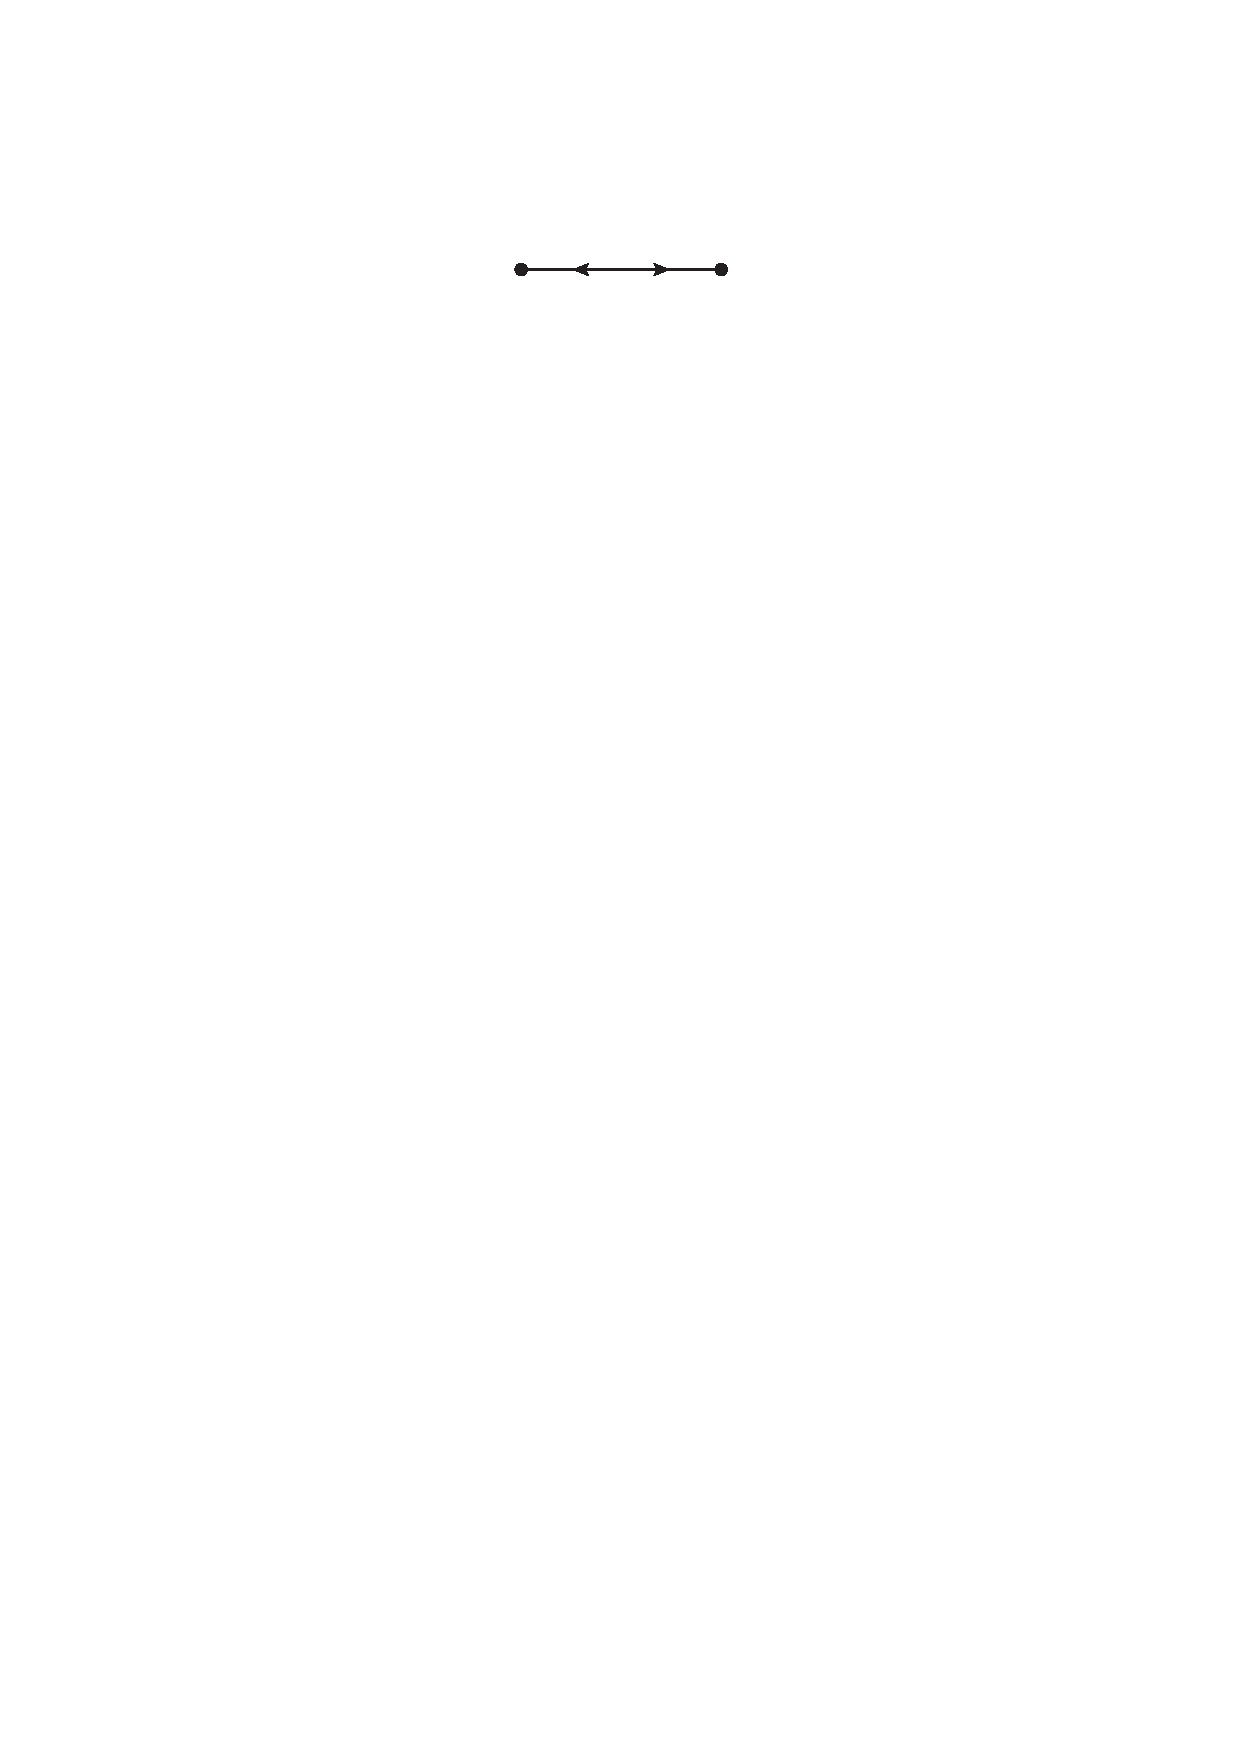
\includegraphics[scale=1]{../pics/majo2.pdf}
\end{minipage}
\begin{minipage}{0.45\textwidth}
\begin{flushleft}
\begin{subequations}
\begin{align}
&\frac{\slashed{k}+m}{k^2-m^2}\label{eq_diracprop}\\
 C^{-1}&\frac{(\slashed{k}+m)}{k^2-m^2}\label{eq_majproptowards}\\
 &\frac{(\slashed{k}+m)}{k^2-m^2}C\label{eq_majpropoutwards}
\end{align}
\end{subequations}
\end{flushleft}
\end{minipage}
\\
\noindent where the first one \eqref{eq_diracprop} corresponds to the standard Dirac propagator and the remaining two lead to fermion number 
violating diagrams. In case a Dirac fermion $\psi$ interacts chirally with a Majorana fermion, the action of $C$ reads as \cite{Langacker}
\begin{align}
 \left[\bar\psi \gamma^\mu (1-\gamma_5)\right]_\beta (C)_{\alpha\beta} = \left[(1-\gamma_5)\gamma^\mu \psi^c\right]_\alpha
 \label{eq_DirMaj}
\end{align}
using \eqref{eq_Ctrafo} and \eqref{eq_chiralflip} and with $\alpha$, $\beta$ as spinor indices. 


